\chapter{Experiment}\label{ch.exp}

Having thus formed a clear picture of what observable effects we expect to manifest from our changes to the Standard Model, we can now proceed with the experimental test.

To save time and avoid trademark infringements, this thesis will use the already existing \textsc{atlas}\footnote{\textbf{A} \textbf{T}oroidal \textbf{L}HC \textbf{A}pparatu\textbf{s}.} experiment, which is part of the Large Hadron Collider complex at \textsc{cern}\footnote{\textbf{C}onseil \textbf{E}uropéen pour la \textbf{R}echerche \textbf{N}ucléaire. When the council tasked with creating the european nuclear research laboratory became the organisation tasked with running that laboratory, its name changed to Organisation Européenne pour la Recherche Nucléaire---the European Organisation for Nuclear Research, but the initialism remained. Acronyms, it seems, are not only ubiquitous, but also immutable.} in Geneva.

\section{The Large Hadron Collider}

\begin{figure}[htp]
\begin{center}
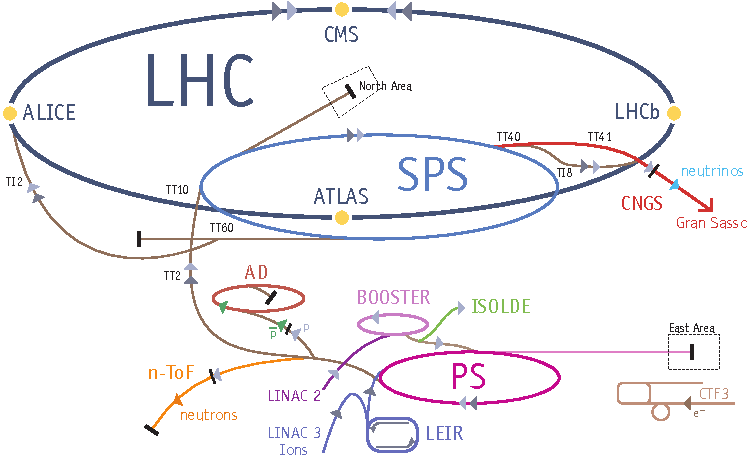
\includegraphics[width=.8\textwidth]{Cernrings}
\end{center}
\begin{minipage}[b]{\textwidth}
\caption{A schematic view of the \textsc{cern} accelerator complex \cite{cernbro}, in which protons or heavy ions used in collision experiments are accelerated through several machines to progressively higher energies. The paths protons can take through the machine are marked with light gray triangles. The dark gray triangles mark the paths taken by heavy ions when the Collider runs proton--lead or lead--lead collision experiments. Protons are `created' by ionising hydrogen atoms and then injected by \textcolor{Purple}{LINAC 2} into the \textcolor{Plum}{Booster ring}. From there, protons are accelerated by the Proton Synchrotron (\textcolor{Magenta}{PS}) and then the Super Protron Synchrotron (\textcolor{RoyalBlue}{SPS}) before finally being sent into the \textcolor{MidnightBlue}{LHC} ring. The LHC ring is the largest circular accelerator in the \textsc{cern} complex, and---at time of writing---in the world, measuring approximately 27~km in circumference.}
\label{cernrings}
\end{minipage}
\end{figure}

The \textsc{cern} accelerator complex comprises a number of particle accelerators with a wide variety of sizes, which service several experiments with various aims \cite{cernexps}. The most conspicuous element of the accelerator complex, of which an overview is given in figure~\ref{cernrings}, is the LHC ring, which is 27~km in circumference (which, even by the standards of particle accelerators, is quite large) and designed to contain proton (a species of hadron) beams with energies as high as 7~TeV. Where two such beams cross one another, proton collisions with 14~TeV energy may occur. The LHC's beams cross one another at four points around the ring, each one the site of one of the four main experiments.

The LHC is the last step in a series of particle accelerators---which incorporates two of \textsc{cern}'s previous main accelerators, the Proton Synchrotron and the Super Proton Synchrotron---which is needed to bring protons from rest to a final energy of 7~TeV. Throughout, protons are accelerated by applied electric fields, applied within so--called radiofrequency cavities, and contained within the rings by dipole magnets. Magnets with higher pole counts are used to manipulate the profile of the proton beam. [Fernow, maybe?]

Even though the LHC was designed for an energy per beam of 7~TeV, giving a collision energy of 14~TeV, several accidents during commissioning of the machine have necessitated the use of a lower beam energy for the first runs. In 2012, when the data that will be used in this thesis was taken, the LHC ran at 4~TeV per beam, for a total collision energy of 8~TeV.

Although we speak of proton beams, protons within the beams are arranged in discrete bunches, occurring at 50~ns intervals. As a consequence, proton collisions occur only within known time intervals, which dictate the timing by which detector readout occurs.

\section{The ATLAS detector}
The \textsc{atlas} detector is the largest of the LHC's four detector expermients, and is, as is the CMS\footnote{The \textbf{C}ompact \textbf{M}uon \textbf{S}olenoid.}, a general purpose detector, designed to capture as much information as possible about collision events. To that end, the \textsc{atlas} detector is made up of three distinct detector subsystems, layered concentrically about the interaction point, as illustrated in in figure~\ref{allatlas}. From innermost to outermost, these are: the tracking system, the calorimeter system and the muon spectrometer.

\begin{figure}[htp]
\begin{minipage}[b]{.69\textwidth}
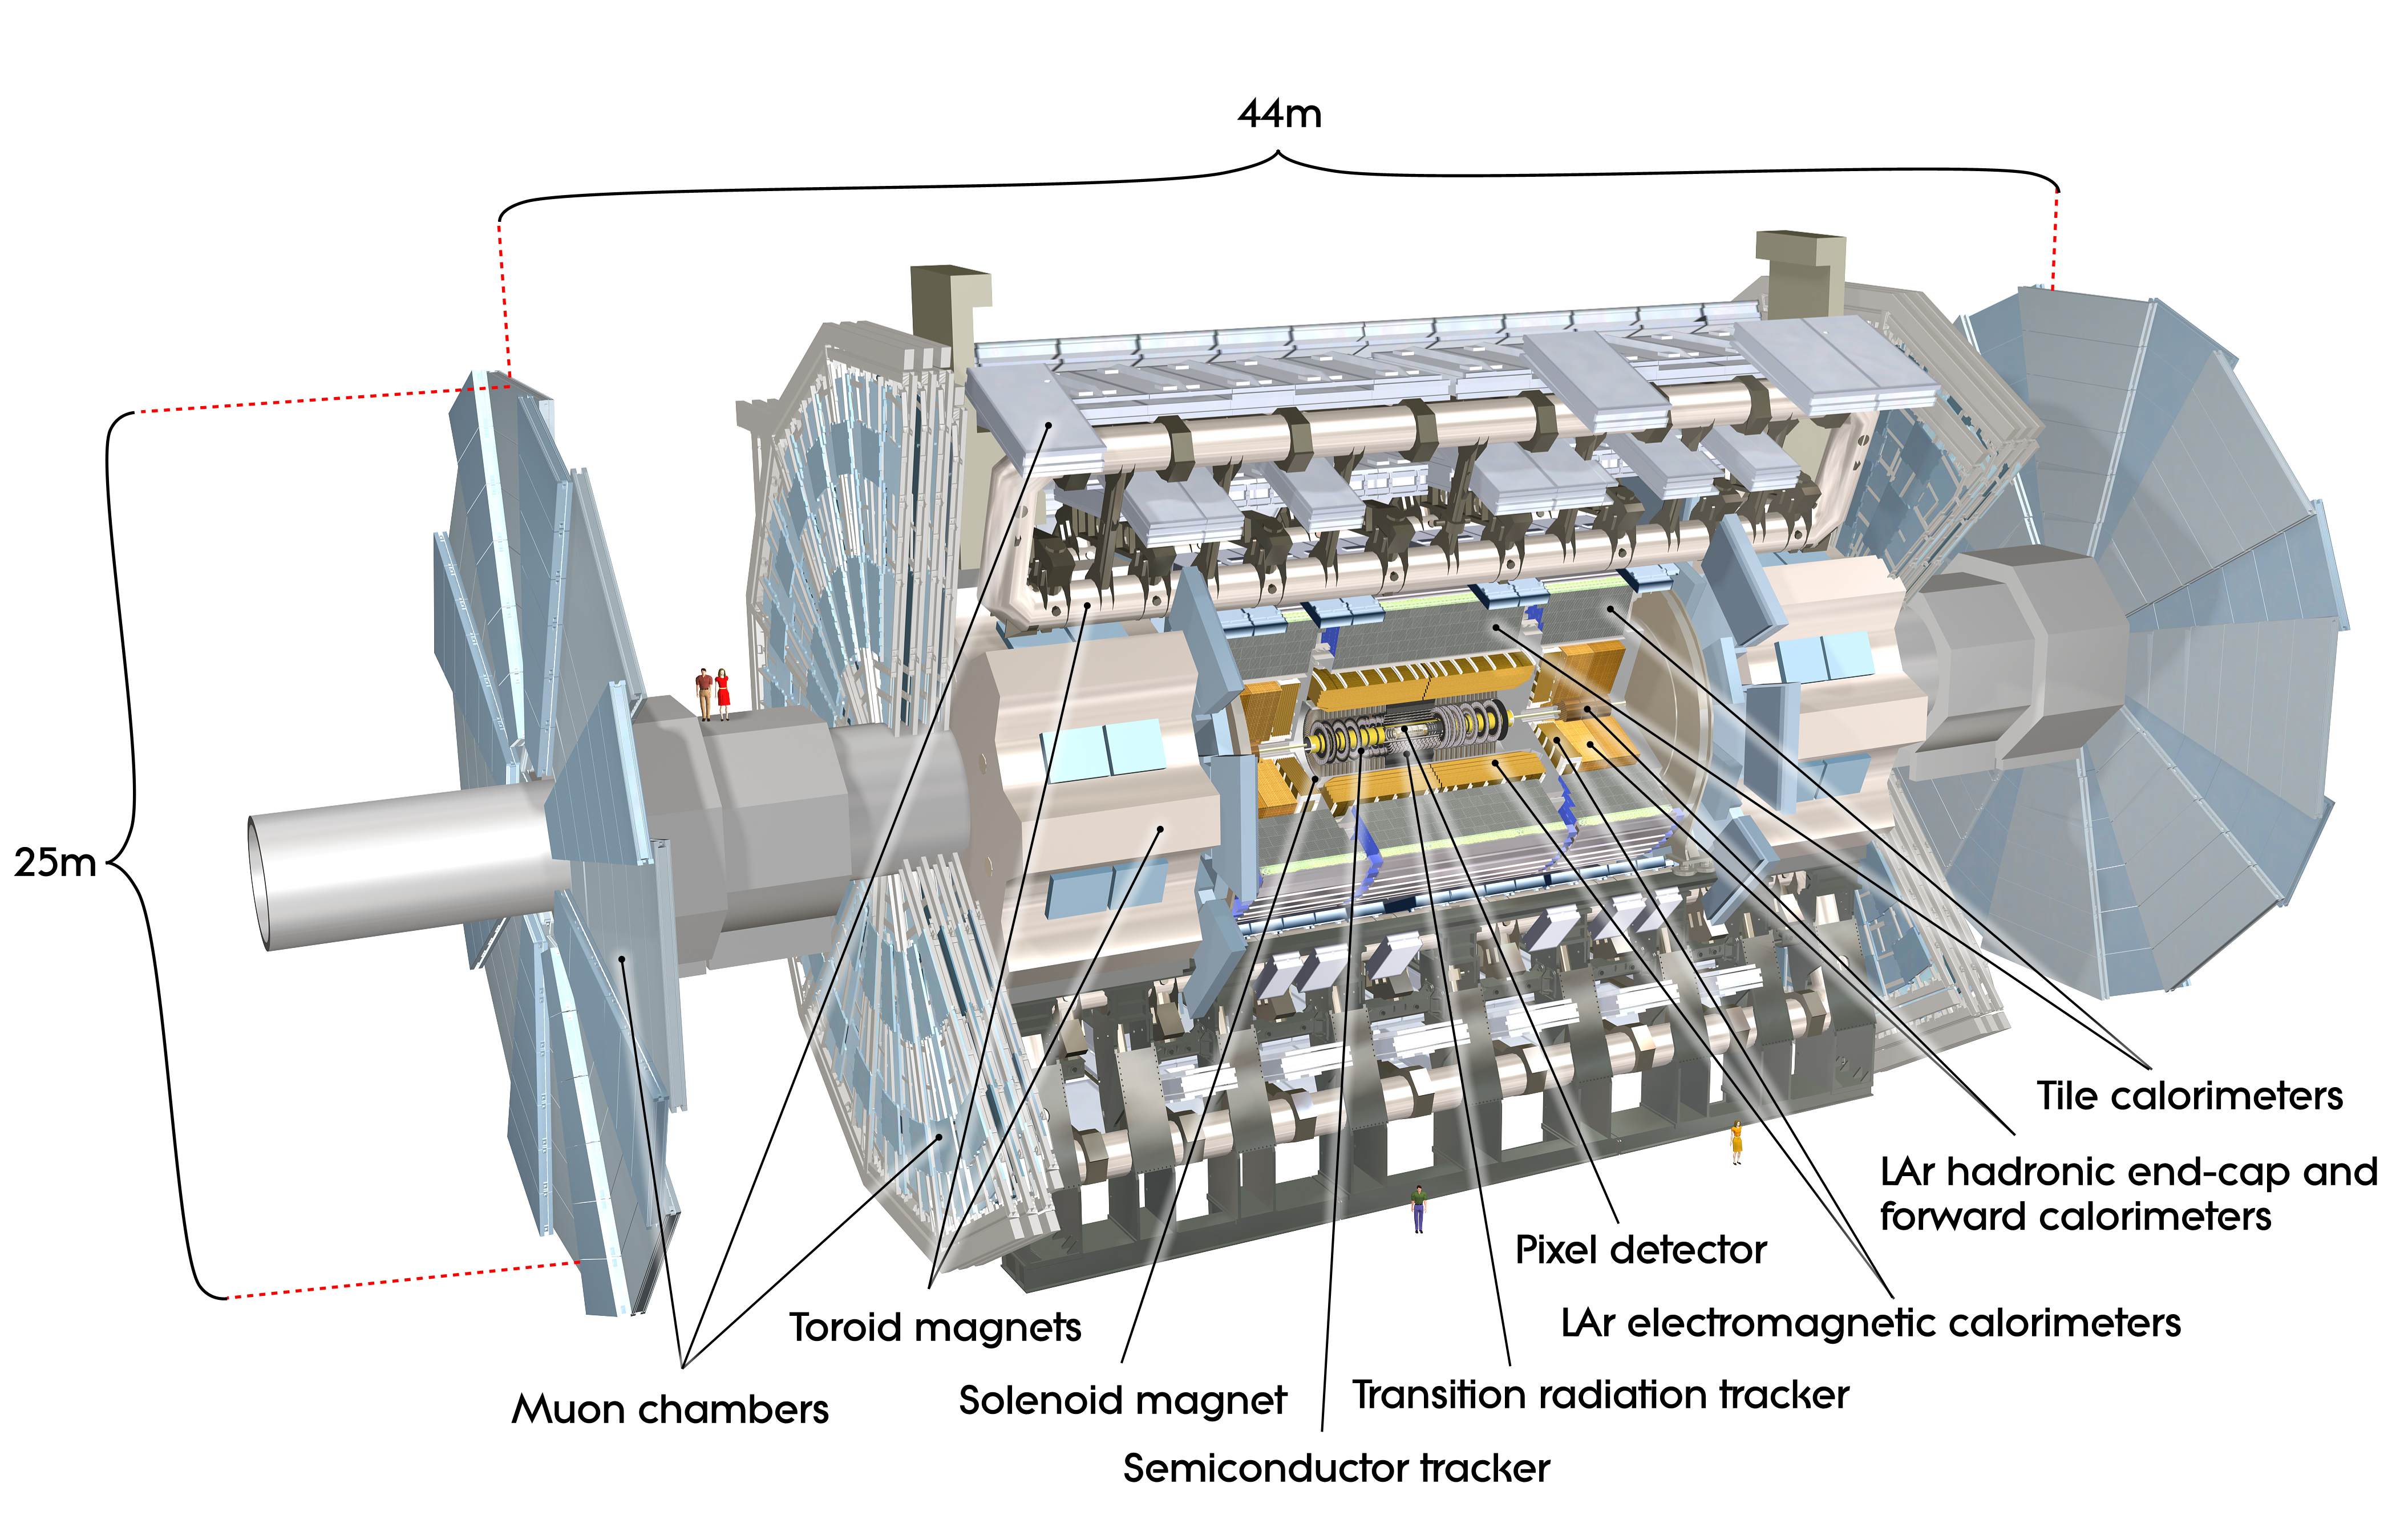
\includegraphics[width=1\textwidth]{AllAtlasBig}
\end{minipage}
\begin{minipage}[b]{.3\textwidth}
\caption{A diagram of the full \textsc{atlas} detector \cite{atlasweb}. The overall structure is of a layered cylinder centred on the interaction point. We refer to those parts of the detector that make up the wall of the cylinder as the barrel section, and to the ends of the cylinder as the endcap. The electromagnetic calorimeter, which is the detector element that we will make the most use of here, is coloured orange in this drawing.}
\end{minipage}
\label{allatlas}
\end{figure}

\textsc{Atlas} defines its own coordinate system, centred on the interaction point, where the position in the angular direction, perpendicular to the beam pipe, is measured by the azimuthal coordinate $\phi$, and the angle to the beam pipe is measured in pseudorapidity $\eta$, which is defined as
\(\eta\equiv-\ln[\tan(\theta/2)]=\half\ln\frac{|\mathbf{p}|+p_z}{|\mathbf{p}|-p_z},\)
where $\theta$ is the polar angle to the beam pipe in radians \cite{green:eta}. The pseudorapidity $\eta$ is a simple transformation of $\theta$---it is 0 at $\theta=\pi/2$, $\infty$ at $\theta=0$ and $-\infty$ at $\theta=\pi$---but is chosen since it is approximately, and for massless particles exactly, equal to rapidity, 
\[ y \equiv \frac{1}{2} \ln \frac{E + p_z }{E - p_z }, \]
which is additive under Lorenz boosts in the $z$ direction \cite{green:y}.

A machine as large and complex as \atlas{} would require a large document, such as~\cite{detectorpaper}, to describe in comprehensive detail. For the present, a decidedly non--comprehensive description of the three detector layers, in order of increasing relevance to this work, follows:

The muon spectrometer forms the outermost, and most voluminous, part of the detector. As a species, muons, along with neutrinos, are the only types of particles that can regularly penetrate both calorimeters. Capturing neutrinos with \textsc{atlas}' mere 90\,000~t of material and 7\,000~m$^3$ detector volume \cite{atlasweb} is something of a lost cause, however.

The muon spectrometer and the inner detector are both tracking detectors, meaning that they are designed to determine the path of a charged particle that passes through them. By immersing such a detector in a magnetic field, which will deflect a charged particle, the charge sign and momentum of the particle can be deduced from the curvature of the track.

The inner detector is also a tracking detector, which uses two distinct detector technologies to localise the tracks of charged particles that pass through it. The innermost layers use silicon semiconductor chips to detect the charge left by a passing charged particle, essentially by allowing the ionisation charge to flip a transistor. The outer part of the inner detector uses drift straws, long tubes with a wire with a high voltage charge in the centre, and filled with an inert gas. The ionisation charge left by a passing high--energy particle is attracted to the wire, and read out by detectors attached to its ends as a voltage change. The silicon detector is compact system with a high resolution, whereas the straw detectors can economically cover a large volume.

Both the straw detector and the outer part of the silicon detector---the silicon microstrip detector---have very long detector elements, which can only report that a hit has occurred somewhere along its length\footnote{Some additional resolution can be gained by studying the drift time in the straw detectors.}. To improve resolution in the long direction of these detectors, successive layers of detector elements are placed at an angle to one another, so that hits on successive detector elements narrow down the possible location of a track. The innermost layer of the silicon detector, the pixel detector, uses a pixel structure rather than a strip structure, and so has adequate resolution in all directions. What is worth noting here is that the tracking detector only directly reports times and---more or less approximate---locations of particle observations. They are only combined into particle tracks during a later analysis step. 

There are two calorimeter systems in \textsc{atlas}: the (inner) electromagnetic calorimeter and the (outer) hadronic calorimeter. In this context, a calorimeter is a device which attempts to absorb energetic particles in some material, and then measures the amount of energy deposited in the process. All calorimeters in \textsc{atlas} are sampling calorimeters, meaning that the absorbing material is divided into layers, with some form of detector inserted between the layers, which sample the flow of energy through the material at various depths. In the barrel section of the hadronic calorimeter---the tile calorimeter, the absorbing material is steel, and the sensitive layers are scintillators, a material that luminesces when exposed to ionising radiation. The light produced there is then guided to photomultipliers for detection.

The remaining calorimeters, which covers both the EM calorimeters and the endcap hadronic calorimeters, are all of a similar design, which has liquid argon as the sensitive material, and are thus called LAr calorimeters. As with the straw detectors, activity in the liquid argon layers are detected by an electrode, which picks up the ionisation left by passing energetic particles. In the barrel LAr calorimeters, the absorbing material is lead encased in thin steel layers. The endcap LAr calorimeters, however, are subjected to much stronger particle fluxes, lead is replaced with copper, and in some cases tungsten, which is more resistant to high temperatures.

\subsection{The electromagnetic calorimeter}

The EM calorimeters are particularly important tools for detecting photons. As such, we devote an entire sub--section to their description.

\begin{figure}[htp]
\begin{minipage}[b]{.69\textwidth}
\begin{infilsf}\footnotesize
\begin{tikzpicture}[x=\textwidth*.95/3.5,y=\textwidth*.95/3.5]

\tikzset{photon/.style={decorate,decoration={snake,amplitude=1}},
         vert/.style={fill=black,circle,draw,inner sep=0pt,minimum size=2},
         grid/.style={draw=kugray!50}
         }
         
\draw[grid] (0,-.6) -- +(0,1.5) (1,-.6) -- +(0,1.5) (2,-.6) -- +(0,1.5) (3,-.6) -- +(0,1.5);
\draw (-.2,-.6) -- (0,-.6) node[below] {0} -- +(0,.05) +(0,0) -- ++(1,0) node[below] {1} -- +(0,.05) +(0,0) -- ++(1,0) node[below] {2} -- +(0,0.05) +(0,0) -- ++(1,0) node[below] {3} -- +(0,.05) +(0,0) -- ++(.3,0);
\draw (3.2,-.6) +(0,-1.1em) node[below left] {Depth in radiation lengths};

\draw (-.1,0) -- (0.4,0) node[vert] {} -- (1.7,-.2) node[vert] {} -- (2.7,-0.1) node[vert] {} -- (3.2,0) ;
\draw[photon] (0.4,0) -- (1.3,.2) node[vert] {};
\draw (1.3,.2) -- node[above] {\tiny$+$} (2.5,.5) node[vert] {} -- node[below] {\tiny$+$} (3.2,.4);
\draw[photon] (2.5,.5) -- (3.2,.7);
\draw (1.3,.2) -- (2.3,.1) node[vert] {} -- (3.2,.2);
\draw[photon] (2.3,.1) -- (3.2,.05) (2.7,-.1) -- (3.2,-.1) (1.7,-.2) -- (2.3,-.3);
\draw (3.2,-.3) -- (2.3,-.3) node[vert] {} -- node[below] {\tiny$+$} (3.2,-.5);



\end{tikzpicture}
\end{infilsf}
\end{minipage}\hfill
\begin{minipage}[b]{.3\textwidth}
\caption{A schematic description of an EM shower developing in an absorbing material, adapted from \cite{fernow:sampcal}. Here, a wavy line indicates a photon, a straight line indicates an electron, and a straight line with a `$+$' a positron. At each split, the two resulting particles carry away half the energy of the original particle. In a sampling calorimeter, a sensitive layer is typically inserted at intervals of one radiation length. \textsc{Atlas}' LAr calorimeters measure the magnitude of ionisation that is left in the liquid argon by the passage of the particle shower.
\label{emshower}
}
\end{minipage}
\end{figure}

In the presence of matter, high--energy photons loose energy primarily through pair production, while electrons loose energy primarily through bremsstrahlung. The typical lengths travelled by both types of particle before undergoing these respective processes---their radiation lengths---depend on the material traversed, but are roughly equal to one another \cite{fernow:sampcal}. As illustrated in fig.~\ref{emshower}, both types of particles will undergo the same sort of evolution as they travel through an absorbing material, splitting into pairs of particles, each with a fraction of the energy of the parent particle, until the daughter particles no longer have sufficient energy to penetrate the absorbing material. Within the calorimeter, this cascade of particles forms a shower structure, an example of which is sketched in fig.~\ref{shower}. Thus, we can measure the energy of the original particle both by how deep into the absorbing material it penetrates, and by how many daughter particles it produces. In a homogeneous calorimeter, such as the one in CMS, where a single material is used both for absorbtion and detection, only the amount of activity produced by a hit to the calorimeter is measured. In a sampling calorimeter, where the absorbing material is passive, and activity is sampled by inserting sensitive layers into the absorbing material at intervals, can measure both the penetration depth, since the thickness of absorbing material in front of the deepest activated sensitive layer is known, and showering activity, by using proportional detectors in the sensitive layers. The radiation length is then a natural choice for the thickness of each layer of absorber.

\begin{figure}[htp]
\begin{minipage}[t]{.4\textwidth}
\caption{Several figures, from \cite{atlasweb}, that illustrate the structure and use of the LAr calorimeters. These are sampling calorimeters, which have an absorbing medium (primarily lead and steel) with layers of detecting medium (liquid argon) inserted regularly to measure particle flux. In \textsc{atlas}' LAr calorimeters, rather than having flat layers, the absorbing and sensitive materials are interleaved in an accordion shape, visible in \subcaptionref{larpic} and \subcaptionref{shower}, which allows the detector electronics to be inserted along the gaps between the absorbing plates. Thus, the calorimeters do not need to be interrupted by non--sensitive space for signalling connections.
\label{calostruc}}
\end{minipage}\hfill\begin{minipage}[t]{.57\textwidth}
\phantom{p}

\phantom{p}

    \begin{center}
    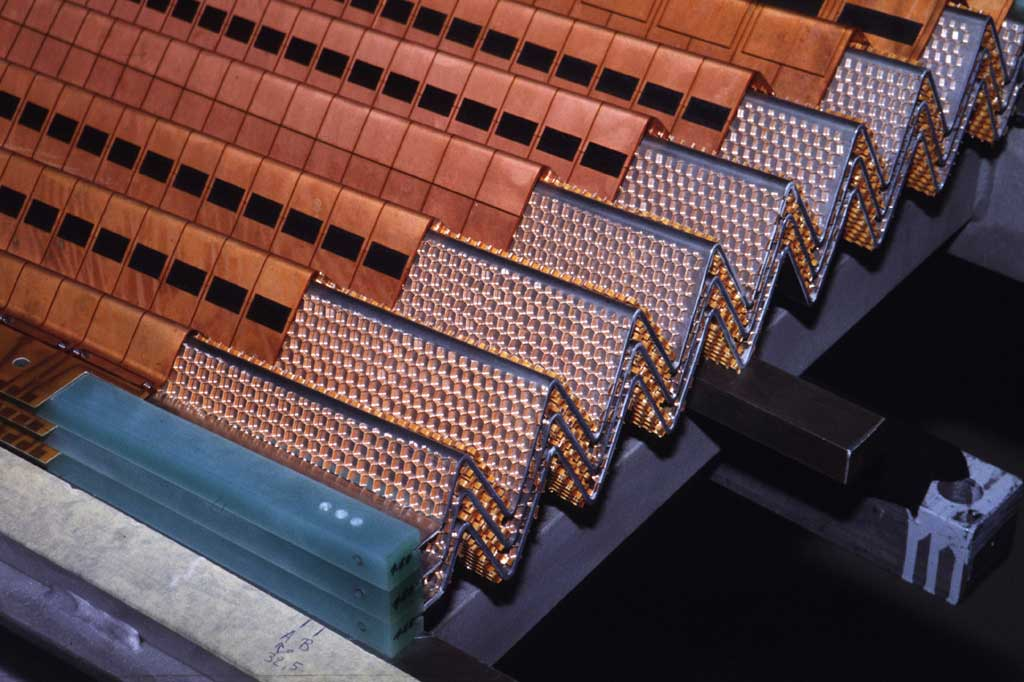
\includegraphics[width=\textwidth]{larpic}\makebox[0em][r]{\textcolor{natgreen}{\rule{\textwidth}{1pt}}}
    
    \contsubcaption{A section of the LAr calorimeter. \label{larpic}}
    \end{center}
\end{minipage}

\noindent\begin{minipage}[b]{.4\textwidth}
\begin{center}
    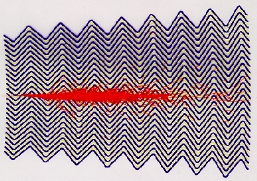
\includegraphics[width=\textwidth]{shower}\makebox[0em][r]{\textcolor{natgreen}{\rule{\textwidth}{1pt}}}

    \contsubcaption{Illustration of a particle shower within the LAr calorimeter. \label{shower}}
    \end{center}
\end{minipage}\hfill\begin{minipage}[b]{.57\textwidth}

    \begin{center}    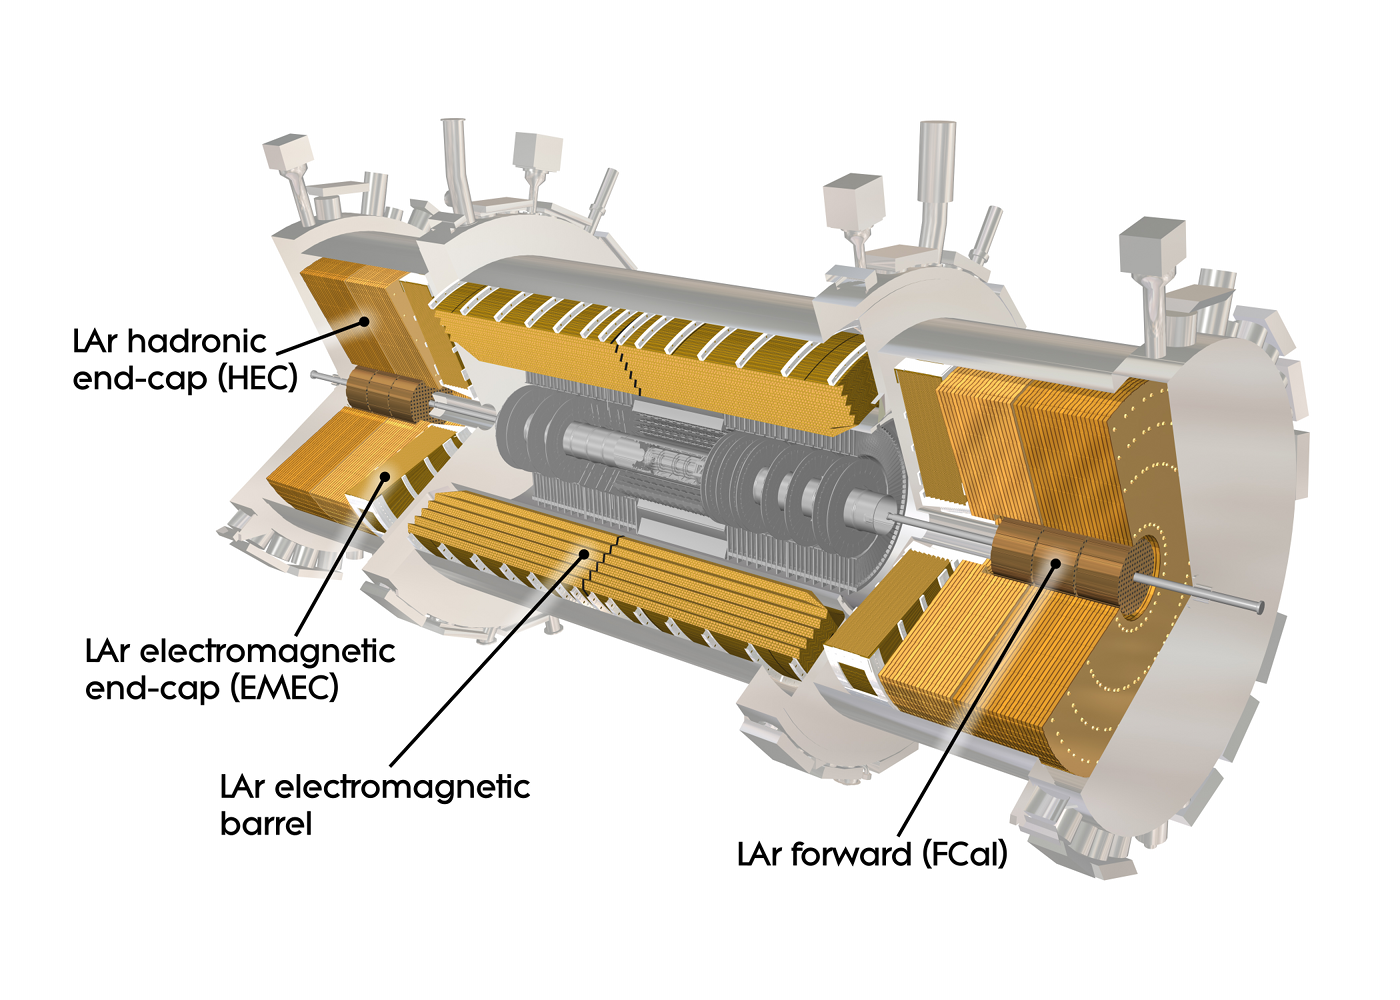
\includegraphics[width=1\textwidth]{figures/CaloDiag.png}
    \contsubcaption{Schematic showing the placement of the LAr calorimeters in \textsc{atlas}.}
    \end{center}
\end{minipage}
\end{figure}

\Atlas{}' barrel LAr calorimeters are divided into three layers, which are split into readout bins as illustrated in fig.~\ref{caldiv}. The first layer is very finely divided in the $\eta$ direction, and its readout cells will on occasion be referred to as `strips' in the `strip layer', as opposed to the `cells' in the other two layers. The detectors function on the same sort of principle as the straw detectors in the inner detector: charged particles leave ionisation trails in the liquid argon, which is picked up on plates suspended in the middle of the LAr gap, which carry a high voltage charge. Each cell functions as a single proportional counter. Thus, the amount of energy deposited in each cell of each layer of the calorimeter is measured by the amount of showering activity in the sensitive layers of that cell.

\begin{figure}[htp]
\begin{minipage}[b]{.69\textwidth}
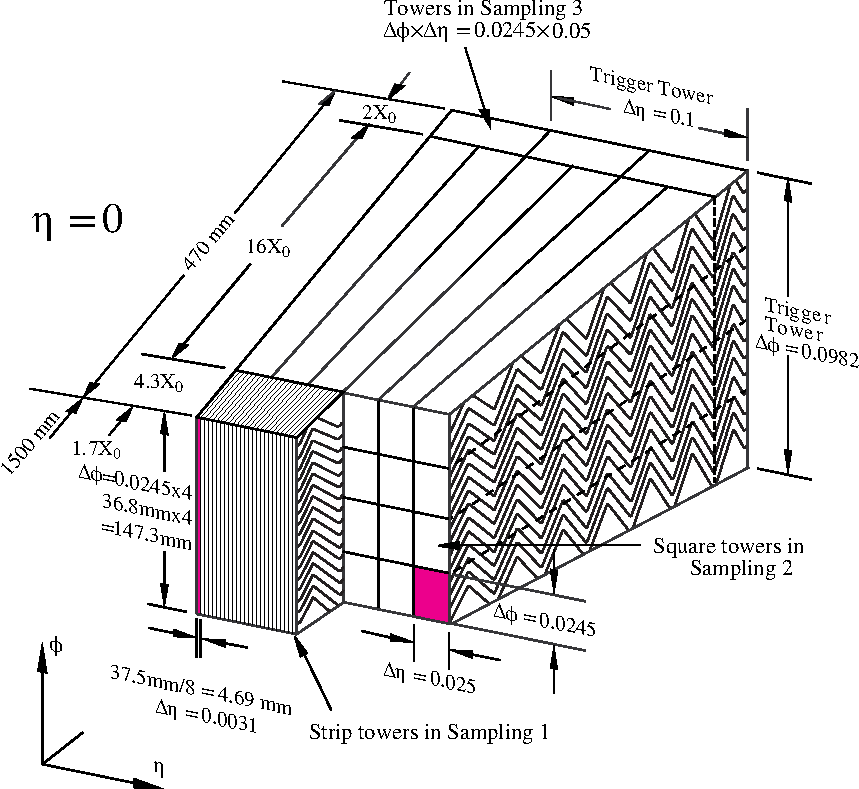
\includegraphics[width=\textwidth]{caldiv}
\end{minipage}
\begin{minipage}[b]{.3\textwidth}
\caption{The division of the EM calorimeter into detecting cells \cite{egede}. The first layer is divided into thin strips for the greatest resolution in the $\eta$ direction. The second layer is divided into roughly square cells, and comprises the bulk of the depth of the detector. The last layer is presumed to only be reached by the most energetic particles, and can have a coarser division without loosing resolution. This diagram is of the calorimeter at $\eta = 0$, closest to the interaction point. At higher $|\eta|$, the towers are angled so that they are still pointed toward the interaction point.
\label{caldiv}}
\end{minipage}
\end{figure}

The absorbing material in the barrel LAr calorimeter are accordion shaped sheets of lead held in iron sheets, visible in fig.~\ref{calostruc}, inserted radially into the detector, so that radiation leaving the detector is still faced with broadly uniform layers of absorbing material, while gaps between them, which are filled with liquid argon and hold the detector plates, still run contiguously throughout the depth of the calorimeter. Connections between the detectors in the inner part of the calorimeter and the readout electronics outside the calorimeter can be run through these gaps without needing to create holes in the detectors coverage.

The division of the calorimeter into layers gives us some resolution in depth when attempting to ascertain the shape of a shower. Showers initiated by types of particles other than photons or electrons evolve in a slightly different way, which allows us discern the source of a shower by examining its shape. Additionally, with this shower shape information, we can extrapolate the direction from which a particle entered the calorimeter, which is of particular importance when attempting to trace the origin of unconverted photons, which otherwise leave no trail in the detector.

There is quite a bit of material between the calorimeter and the interaction point, any of which may interact with a particle in the same way as the absorbing material in the calorimeter. To attempt to correct for this, the first active layer, called the presampler, sits ahead of the first absorbing layer. Photons that undergo pair production sufficiently deep in the detector for the tracker to resolve at least one of the resulting (anti--)electrons are treated as a separate object type, namely converted photons. Identifying all the detector signatures that may have been left by photons is the first major (relevant) step in analysing the detector's output.

\subsection{Photon identification}
In broad terms, we may view information coming from the detector in terms of energy clusters in the calorimeters or tracks in the inner detector. Assigning calorimeter deposits to discrete clusters is a task that can be approached a number of ways, both subtle and complex, however at the photon ID stage, the straightforward sliding window method is used \cite{atlascluster:sw}. A rectangle of fixed size is defined by combining calorimeter cells, and the energy within is summed. This `window' is then `slid' across the entire calorimeter, and a cluster candidate is proclaimed whenever the energy within the window reaches a local maximum above a predefined threshold value.

Assuming that every charged particle leaves both a track in the inner detector and a cluster in the calorimeter, we interpret every cluster in the calorimeter that can not be associated with a track as the signature of a neutral particle. Each of these neutral particles might be an unconverted photon, and so every cluster without an associated track is added to the list of photon candidates.

As previously mentioned, converted photons are photons that undergo pair production ``in flight.'' As such, we expect the detector signature of such events to be a positively and a negatively charged track with a common vertex away from the interaction point. Any set of measurements that match this signature may be added to the sequence straight away, however since track reconstruction is an imperfect process, especially in the straw detector, we include also any electron candidate, whose track is reconstructed solely from hits in the straw detector.

These steps form a selection algorithm, which creates a list of photon candidates for every event in \atlas{} \cite{phorec}.

This set will of course contain many events that were not photons: $\pi^0$ mesons also create calorimeter hits with no associated track, and QCD jets can mimic converted photons, among other possibilities. To attempt to sort genuine photon events from impostor events, we study the shape of the shower left in the calorimeter. To that end, we define the following shower shape variables:

\begin{itemize}
\item $R_\text{had}$, the ratio of energy deposited in the hadronic calorimeter to the cluster energy in the EM calorimeter. Hadronic showers are expected to penetrate deeper into the hadronic calormieter than EM showers.
\item In the middle EM calorimeter layer, non-EM showers spread wider than electromagnetic ones. The variables that measure the shape of the shower in this layer are:
\begin{itemize}
\item $R_\eta$, the ratio in $\eta$ of cell energies in 3 $\times$ 7 versus 7 $\times$ 7 cells.
\item $R_\phi$, the ratio in $\phi$ of cell energies in 3 $\times$ 7 versus 7 $\times$ 7 cells.
\item $w_{\eta 2}$, the width of the shower in the $\eta$ direction.
\end{itemize}
\item The strip layer, with its greater resolution in $\eta$, can pick out some of the internal structure of a jet. Hadron showers tend to show more than one maximum. Variables that measure the shape in the strip layer are:
\begin{itemize}
\item $w_{s3}$, the shower width for three strips around the maximum strip.
\item $w_{s\text{ tot}}$, the total lateral shower width in the strip layer.
\item $F_\text{side}$, the faction of energy deposited outside a core of 3 central strips, but within 7 strips.
\item $\Delta E$, the difference in energy of the strip with the second largest energy deposited and the strip with the smallest energy deposited between the two leading strips.
\item $E_\text{ratio}$, the ratio of the energy difference associated with the
largest and second largest energy deposits, over the sum of these energies.
\end{itemize}
\end{itemize}

Cuts made in these variables form the selection criteria that are used to divide the sample of photon candidates into those that are to be considered actual or impostor photons. The full list of variables above forms the tight selection criteria, while a shorter list, consisting of $R_\text{had}$, $R_\eta$ and $w_{\eta2}$ form the loose selection criteria. Separate cut values in these variables exist for different $\eta$ ranges. A complete description is available in \cite{Carminati}.

\subsection{Triggering and readout}
While in full operation for the 2012, 8~TeV run, the LHC delivered a bunch crossing in \textsc{atlas}' interaction point every 50~ns, or 20 million events per second. Reading out the whole detector produces 1.6~MB of information, which, if the detector were read out completely with every crossing, would produce a data rate of 34~TB/s.\footnote{For perspective, that is approximately equal to the estimated global IP traffic rate in 2015, according to \cite{wolframip}.} However, since only a fraction of these collisions produce interesting physics events, we can reduce the data rate to less prohibitive levels simply by not recording data from collision that do not produce interesting events. To accomplish this, we need a system that examines events in the detector as they occur, and trigger recording whenever it sees an interesting event. In \textsc{atlas}, this trigger system has three levels, which are described in detail in \cite{detectorpaper}. 

The level--1 trigger examines events in real time as they occur in the detector. To do so, the trigger logic is run on specialised hardware built in to the detectors. As a result, each trigger only has access to information from the detector its hardware is attached to. Chalorimeter triggers, for example, do not have access to information from the tracking system at the first trigger level. Also, computationally intensive tasks, such as track reconstruction, can not be completed in the window of time available to the level--1 trigger, and so are also not available. The next trigger level, level--2, is run on the full set of information from an event, on those events which pass the level--1 filter. The final trigger level works with fully reconstructed events and derived physical observables. This requires more time and processing power than is available at the previous levels, but it also identifies interesting events with the same quality of information as will be used in the subsequent analysis. All three triggers in combination cuts the final event rate to 300 events per second, with a peak rate of 600 events.

For this thesis, we shall use data taken during the 8~TeV run in 2012. The amount of data taken at any given time depends on the conditions of the beam, which can be summarised in the instantaneous luminosity, and the conditions of the detector, which may only capture a fraction of the events produced at any given time. Figure~\ref{intlumi} gives the distribution of integrated and captured luminosity over the course of the year.

\begin{figure}[htp]
\begin{minipage}[b]{.57\textwidth}
\hspace{-1em}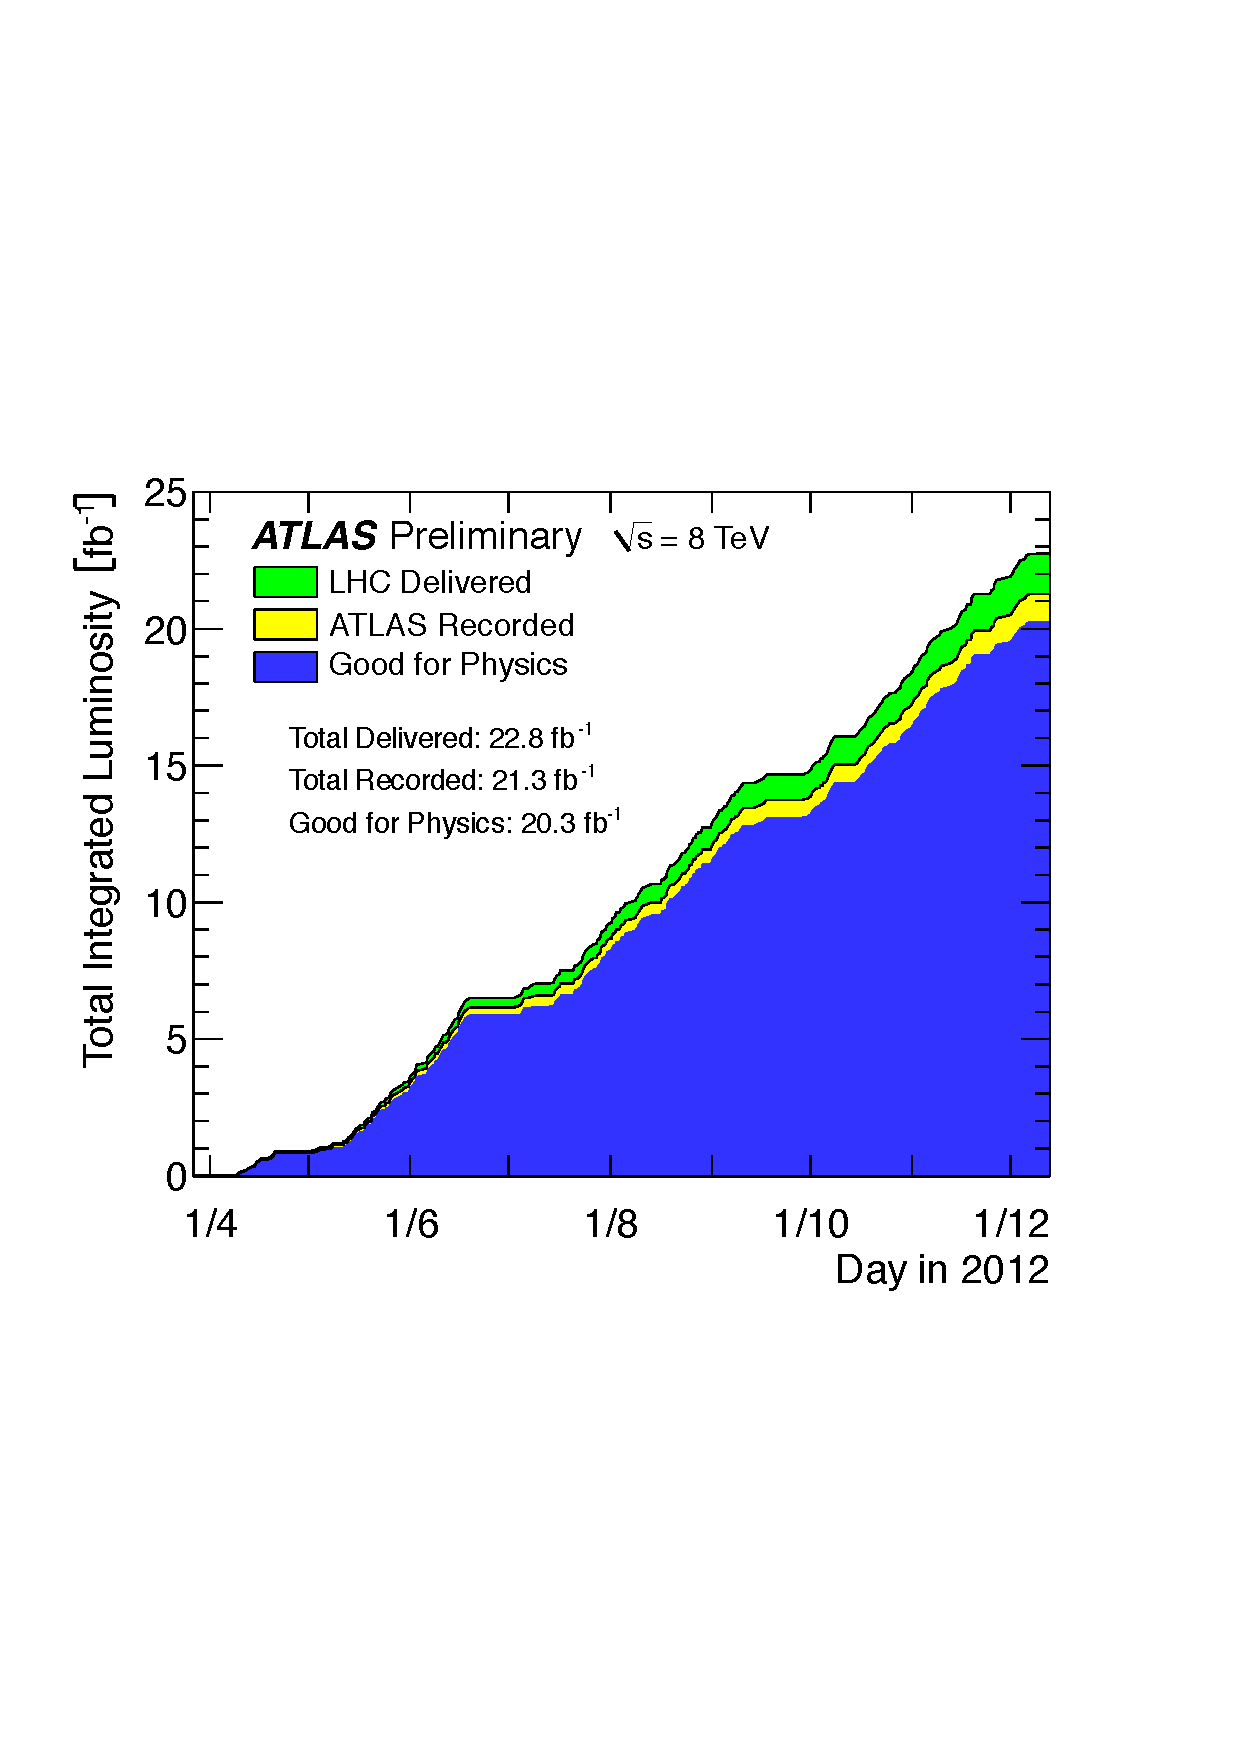
\includegraphics[width=\textwidth]{figures/intlumi}
\end{minipage}\hfill\begin{minipage}[b]{.4\textwidth}
\caption{A plot \cite{publiclumi} showing the integrated luminosity delivered by the LHC (green), recorded by \atlas{} (yellow), and fulfilling data quality criteria (blue), over the course of the 8 TeV run in 2012.
\label{intlumi}}
\end{minipage}
\end{figure}

Unfortunately, the triggers that are implemented in \atlas{} do not guarantee that the event rate remains within the technical limitations of the readout system. To stay within those limits, \atlas{} prescales certian triggers, when they originate from a trigger that produces more events than it is considered worth keeping,\footnote{Explaining how it is decided whether data is worth keeping would veer into a discussion of \atlas{} internal politics, which is a topic beyond the scope of this thesis.} which means simply that a fraction of event that pass a trigger are not recorded. The diphoton channel is important to the search for the Higgs boson, however, so the triggers that produce diphotons events have not been prescaled.
